\section{Dynamics of a Single Cell}
In this section the results of the numerical solutions for a single cell
using the three models presented above are discussed. All results were
obtained with a simple Forward-Euler scheme.


\subsection{Hodgkin \& Huxley}
The equations were integrated for \SI{10}{\milli\second} with a time step
$\Delta{t}=\SI{.01}{\milli\second}$ (\ie~1000 integrations steps) and an
initial potential $V_0=\SI{-7}{\milli\volt}$. The resulting action potential,
current densities and gating variables are plotted in \figref{fig:hh1}.

\begin{figure}[h]
    \centering
    \begin{subfigure}[h]{.3\textwidth}
        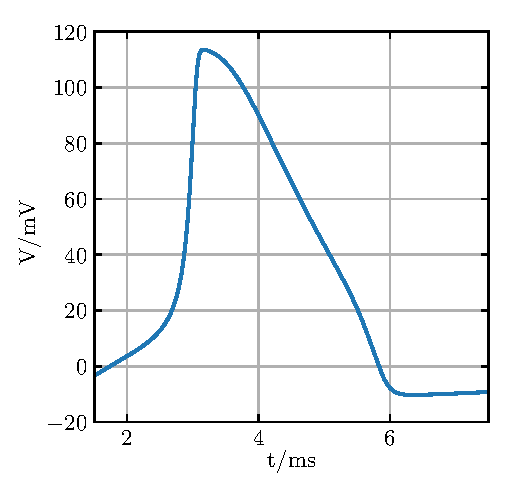
\includegraphics[width=\textwidth]{hh52-10ms-V}
        \vspace{-\baselineskip}
        \label{fig:hh1V}
        \caption{Potential}
    \end{subfigure}
    \begin{subfigure}[h]{.3\textwidth}
        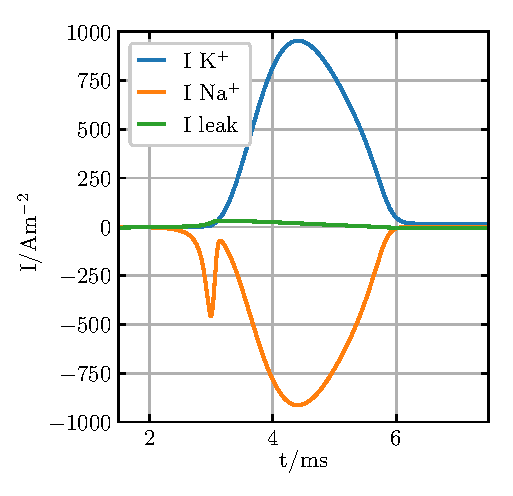
\includegraphics[width=\textwidth]{hh52-10ms-I}
        \vspace{-\baselineskip}
        \label{fig:hh1I}
        \caption{Current Densities}
    \end{subfigure}
    \begin{subfigure}[h]{.3\textwidth}
        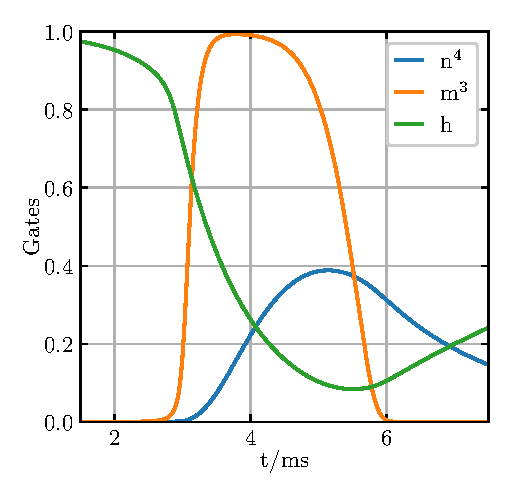
\includegraphics[width=\textwidth]{hh52-10ms-Gates}
        \vspace{-\baselineskip}
        \label{fig:hh1Gates}
        \caption{Gating Variables}
    \end{subfigure}
    \label{fig:hh1}
    \caption{Results of integrating the H\&H model}
\end{figure}

The gating variables were initially all set to 0, yet at
$t=\SI{0}{\milli\second}$ the \ce{Na+} gate $h$ jumps directly to being almost
completely open ($h(t=0)=0.99$); however, the \ce{Na+} current is at this point
suppressed by the closed $m$ gate. The $h$ gate slowly closes up to
$t\approx\SI{5}{\milli\second}$ and then swings down more rapidly, while at the same
time the $m$ gate opens strongly and allows for influx of \ce{Na+} ions
(interesetingly yhe \ce{Na+} current exhibits a small seperate peak at
$t\approx\SI{5}{\milli\second}$ before rising up to its full strength). This
causes the membrane potential to rise up and become strongly positive. Shortly
after the quick opening of the $m$ gate, the \ce{K+} gate $n$ also opens,
allowing for an opposed \ce{K+} outflux causing the membrane potential to
eventually repolarize.

The resulting action potential resembles qualitatively the results depicted in
fig.~12 in [HH52] \todo{add paper to literature and cite properly}. An even
better fit is achieved when integrating the system for \SI{40}{\milli\second}
with and initial value of $V_0=\SI{-30}{\milli\volt}$, as depicted in fig.~22
in [HH52] (see \figref{fig:hh2}).

\begin{figure}[h]
    \centering
    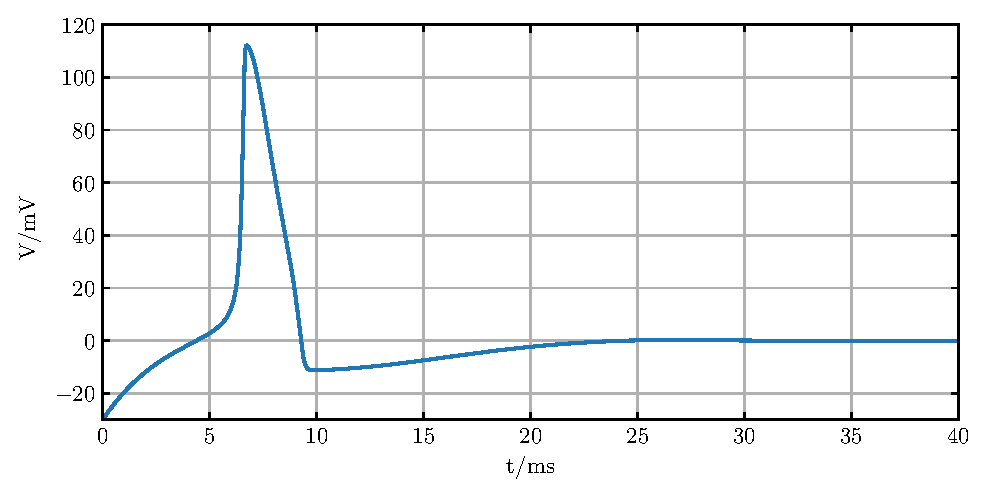
\includegraphics[width=.75\textwidth]{hh52-40ms}
    \label{fig:hh2}
    \caption{H\&H for \SI{40}{\milli\second}; note the hyperpolarization}
\end{figure}

Another interesting effect can be observed when adding an additional source
current density to equation \eqref{eq:cap}, \ie:
\begin{equation*}
    C\,\dv{V}{t}=-\sum_{s}I_{s} + I_{\mathrm{source}}
\end{equation*}
which causes the membrane potential to depolarize again after repolarization
with a constant rate as depicted in \figref{fig:hh3}. Note, that the cell is
firing with a fixed minimal rate given by $I_{\mathrm{source}}$ (All-or-None
principle).

\begin{figure}[h]
    \centering
    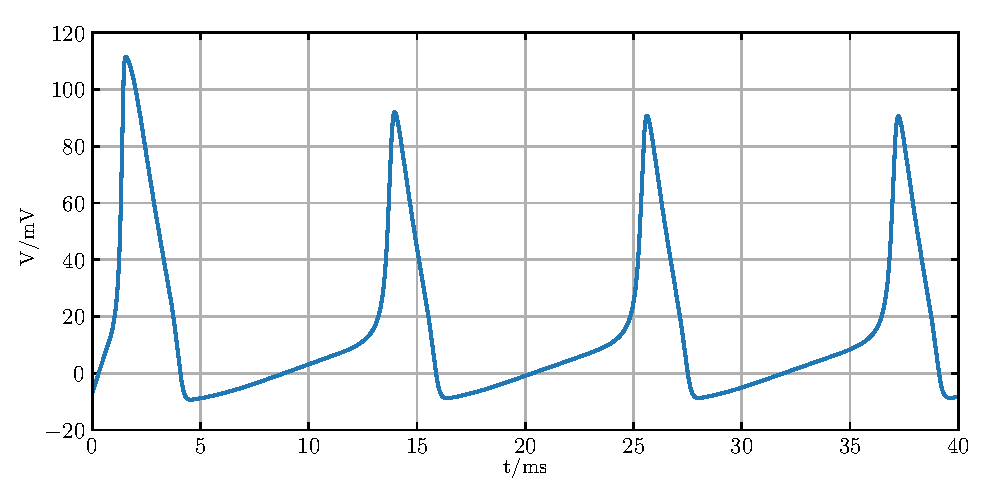
\includegraphics[width=.75\textwidth]{hh52-40ms-10nA}
    \label{fig:hh3}
    \caption{H\&H with
        $I_{\mathrm{source}}=\SI{10}{\ampere\per\metre\squared}$}
\end{figure}


\subsection{Aliev \& Panfilov}
\emph{Note:} The action potential $V$ in this model takes values in $(0,1)$ and
needs to be rescaled according to
$V_{\mathrm{phys}}/\si{\milli\volt}=100\,V-80$. The simulation time $t$ is related
to the physical time via $t_{\mathrm{phys}}/\si{\milli\second}=12.9\,t$.

\vspace{\baselineskip}
The integration was performed for \SI{60}{\stu} (simulationt time units,
\ie~$t_{\mathrm{phys}}=\SI{774}{\milli\second}$) with a time step of
$\Delta{t}=\SI{.01}{\stu}$ (\ie~6000 integration steps) and an initial
excitement of the potential to $V_0=\SI{.2}{svu}$ (simulation voltage
units, \ie~$V_{\mathrm{phys},0}=\SI{-60}{\milli\volt}$).

Upon an excitement which surpasses some threshold, the action potential quickly
raises up to its maximal value. The relaxation variable begins raising, too,
slowly at first, but gradually growing faster until it steeply reaches its
peak, which pulls the action potential back to its resting value.

\begin{figure}[h]
    \centering
    \begin{subfigure}[b]{.45\textwidth}
        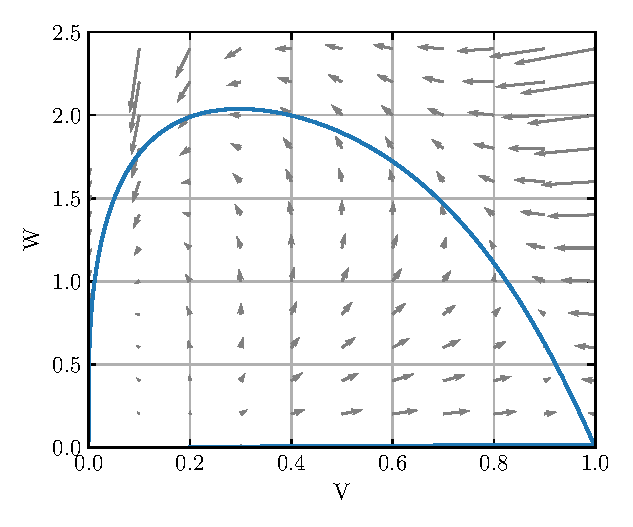
\includegraphics[width=\textwidth]{alpha-phase}
        \vspace{-\baselineskip}
        \label{fig:alphaphase}
        \caption{Phase plot of the system, shows the characteristic connection
        of the two variables (unscaled)}
    \end{subfigure}
    ~
    \begin{subfigure}[b]{.45\textwidth}
        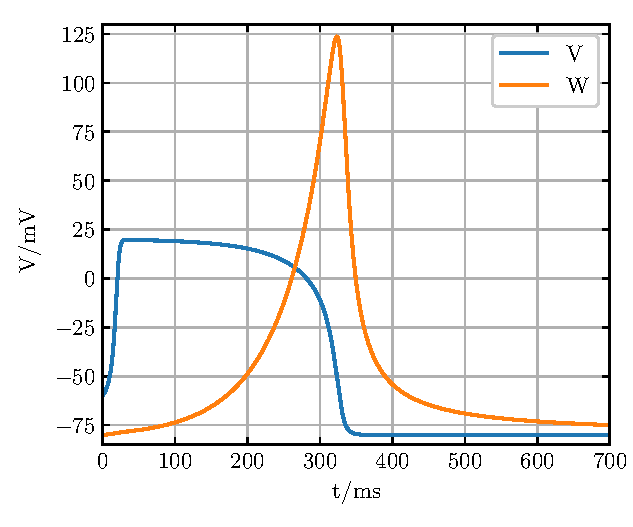
\includegraphics[width=\textwidth]{alpha-dynamics}
        \vspace{-\baselineskip}
        \label{fig:alphadyn}
        \caption{Temporal evolution of two variables (physically rescaled)}
    \end{subfigure}
    \label{fig:alpha1}
    \caption{Results of integrating the A\&P model}
\end{figure}

The model dynamics are governed by a set of five parameteres $a, k, \epsilon_0,
\mu_1\text{ and }\mu_2$. They are phenomenological in their nature and therefor
difficult to interpret. A \_\todo{komprimiert, schnell} study which varies each
parameter while holding the others constant is found in the appendix\todo{ref}.


\subsection{Fenton et al}
\emph{Note:} In this model the action potential also takes values in $(0,1)$
and needs to be rescaled with $V_{\mathrm{phys}}/\si{\milli\volt}=100\,V-80$;
however, the simulation time closely resembles the physical time.

\vspace{\baselineskip}
The integration was performed for \SI{400}{\milli\second} using a time step
$\Delta{t}=\SI{.1}{\milli\second}$ (resulting in 4000 integration steps) and
an initial excitement of the potential $V_0=\SI{.3}{\svu}$
(\ie~$V_{\mathrm{phys}}=\SI{-50}{\milli\volt}$).

The resulting action potential qualitatively resembles the result from the
Aliev-Panfilov model, with the difference that the peak does not start
decreasing right after the excitement but rather shows a slight bump in the
plateau.
Just like the Hodgkin-Huxley model, the Fenton model is  based on an ionic
description, which allows to comprehed the action potential dynamics based on
underlying gate and current processes.

\begin{figure}[h]
    \centering
    \begin{subfigure}[b]{.3\textwidth}
        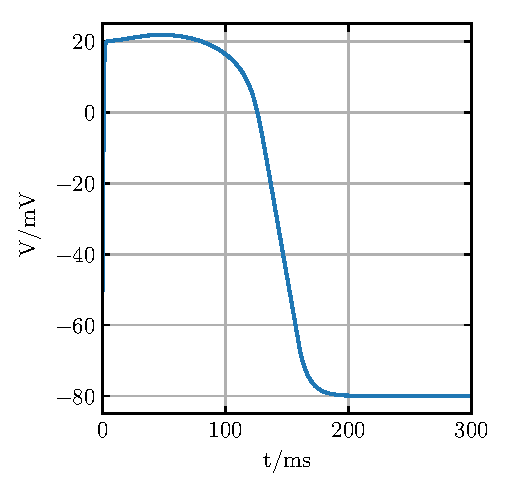
\includegraphics[width=\textwidth]{fenton-single-cell-V}
        \vspace{-\baselineskip}
        \label{fig:fenton1-V}
        \caption{Potential}
    \end{subfigure}
    \vspace{\baselineskip}
    \begin{subfigure}[b]{.3\textwidth}
        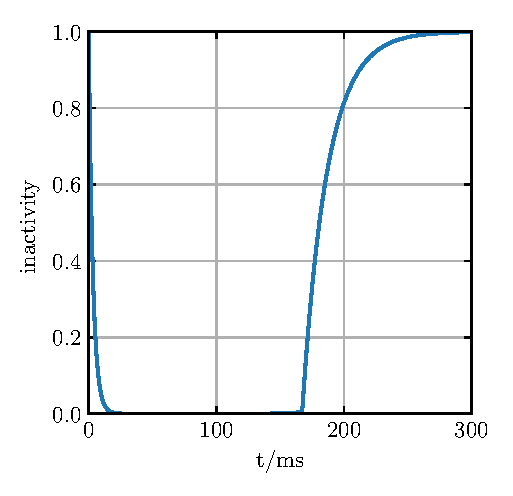
\includegraphics[width=\textwidth]{fenton-single-cell-gate-v}
        \vspace{-\baselineskip}
        \label{fig:fenton1-v}
        \caption{Inactivation gate v}
    \end{subfigure}
    \begin{subfigure}[b]{.3\textwidth}
        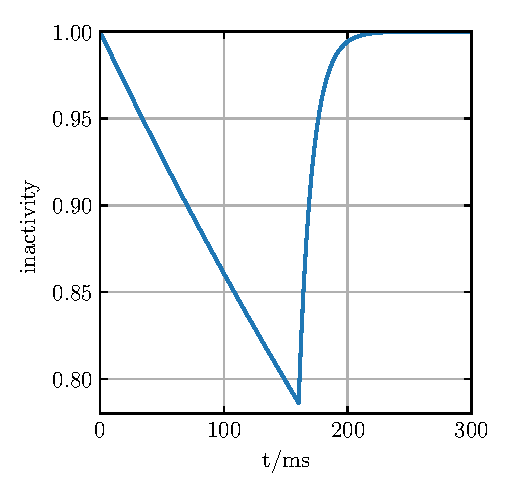
\includegraphics[width=\textwidth]{fenton-single-cell-gate-w}
        \vspace{-\baselineskip}
        \label{fig:fenton1-w}
        \caption{Inactivation gate w}
    \end{subfigure}
    % \vspace{\baselineskip}
    \begin{subfigure}[b]{.3\textwidth}
        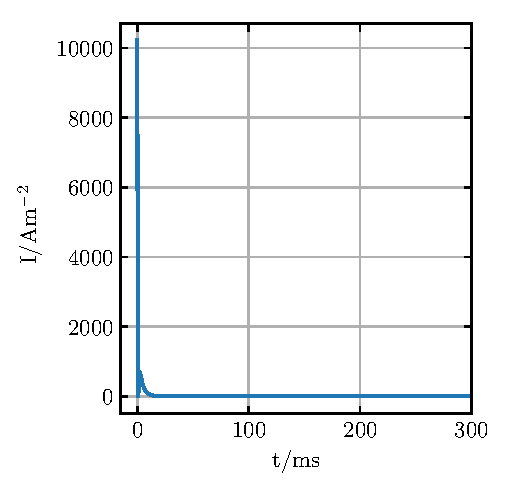
\includegraphics[width=\textwidth]{fenton-single-cell-Ifi}
        \vspace{-\baselineskip}
        \label{fig:fenton1-Ifi}
        \caption{fast inward current}
    \end{subfigure}
    \begin{subfigure}[b]{.3\textwidth}
        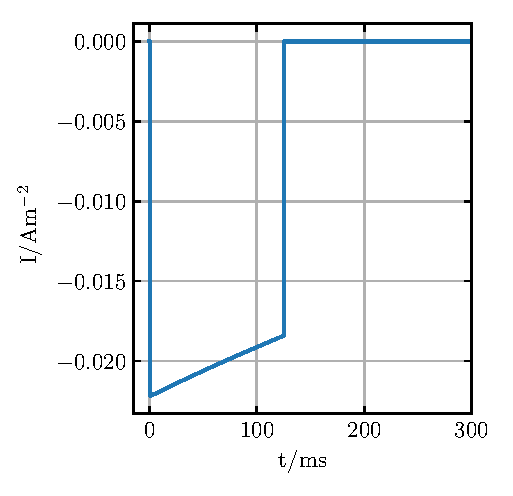
\includegraphics[width=\textwidth]{fenton-single-cell-Isi}
        \vspace{-\baselineskip}
        \label{fig:fenton1-Isi}
        \caption{slow inward current}
    \end{subfigure}
    \begin{subfigure}[b]{.3\textwidth}
        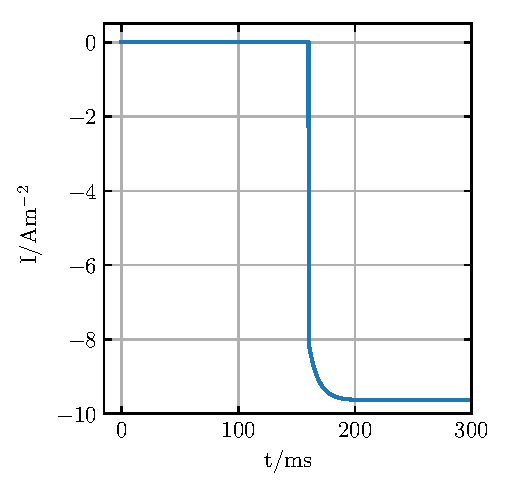
\includegraphics[width=\textwidth]{fenton-single-cell-Iso}
        \vspace{-\baselineskip}
        \label{fig:fenton1-Iso}
        \caption{slow outward current}
    \end{subfigure}
    \label{fig:fenton1}
    \caption{Results of integrating the Fenton model}
\end{figure}

Here are a few things to note:
\begin{itemize}
    \item the gate variables are \emph{inactivation gates}, \ie~1 means fully
        closed, while 0 means fully opened
    \item while the fast inactivation gate $v$ opens completely upon
        excitement and then returns into its closed state, the
        slow inactivation gate $w$ does not open completely (only ca.~21\%)
        before closing again rather quickly.
    \item the currents are modeled with Heaviside-functions in order to be
        activated at once when the potential surpasses a certain threshold
        (given by the parameters $V_c$ and $V_v$); this causes the sudden jumps
        in the plots of the current densities
\end{itemize}


% vim: set ff=unix tw=79 sw=4 ts=4 et ic ai :
